\section{BLDC Motor}
The mathematical model of a BLDC motor is is many ways similar to the one of a conventional DC motor. The main difference is represented by the added phases which affect the resistive and inductive components of the BLDC arrangement.

Therefore, we will start of by describing the mathematical modelling of a DC motor and then change it to fit the BLDC motor.

Figure \label{electromech} illustrates a DC electromechanical system.

\begin{figure}[H]
  \centering
    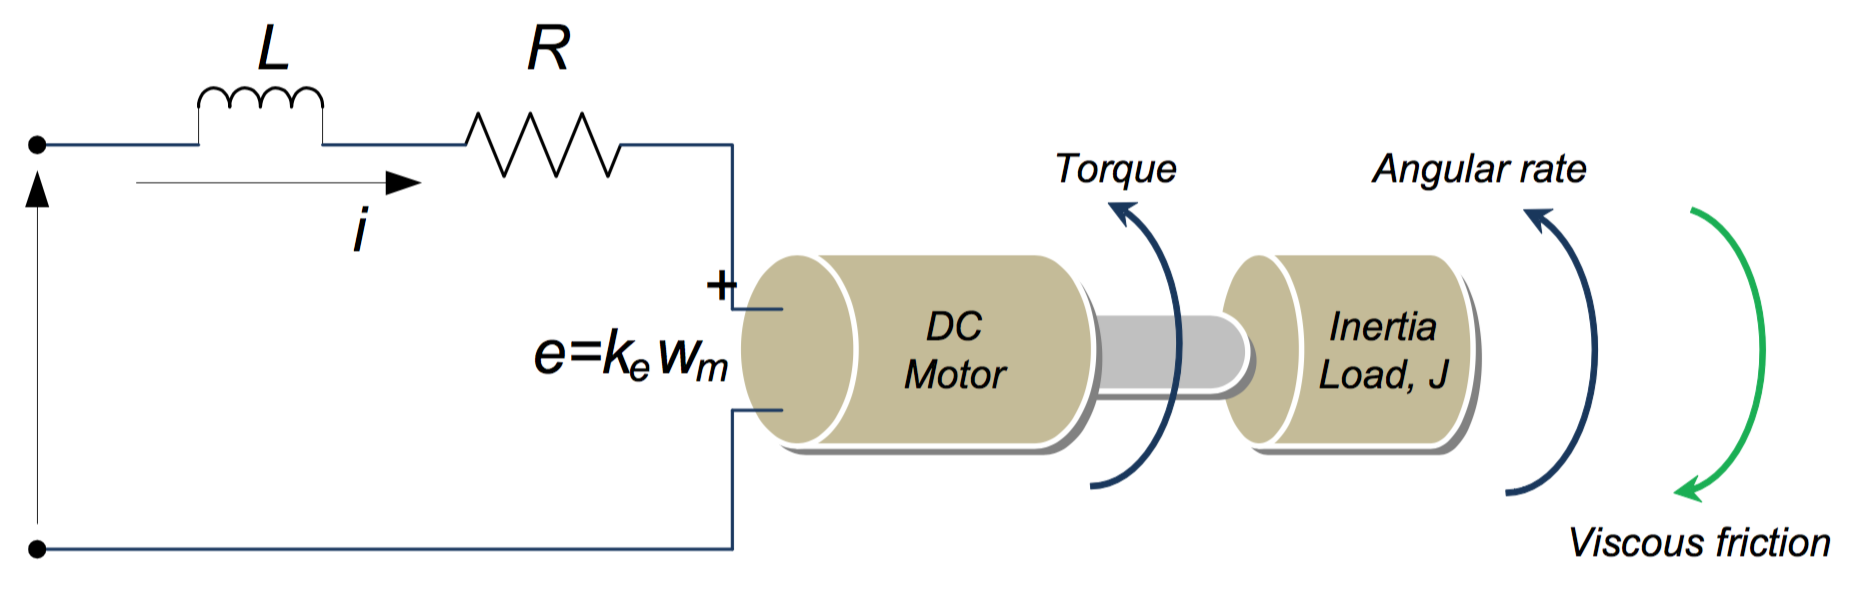
\includegraphics[width=0.9\textwidth]{images/electromech.png}
	\caption{Typical DC electromechanical system}
	\label{electromech}
\end{figure}

The components of the electrical circuit are the armature resistance - R, the armature inductance - L and the back EMF - e. By applying KVL, we obtain:

\begin{equation}
\label{1}
	V_{s}=Ri+L\frac{di}{dt}+e
\end{equation}

where $V_{s}$ - DC source voltage and $i$ - armature current.

Moving on to the mechanical part, further equations can be written using Newton's second law of motion:

\begin{equation}
\label{2}
	J\frac{d\omega_{m}}{dt}=\Sigma{T_{i}}
\end{equation}

\begin{equation}
\label{3}
	T_{e}=k_{f}+J\frac{d\omega_{m}}{dt}+T_{L}
\end{equation}

where $T_{e}$ - electrical torque, $k_{f}$ - friction constant, $J$ - rotor inertia, $\omega_{m}$ - angular velocity and $T_{L}$ - load torque.

The back EMF and the electrical torque can be described as:

\begin{equation}
\label{4}
	T_{e}=k_{t}\omega_{m}
\end{equation}

\begin{equation}
\label{5}
	e=k_{e}\omega_{m}
\end{equation}

where $k_{e}$ - back EMF constant and $k_{t}$ - torque constant.

Rewriting equations \ref{1} and \ref{2} gives:

\begin{equation}
\label{6}
	\frac{di}{dt}=-i\frac{R}{L}-\frac{k_{e}}{L}\omega_{m}+\frac{1}{L}V_{s}
\end{equation}

\begin{equation}
\label{7}
	\frac{d\omega_{m}}{dt}=i\frac{k_{t}}{J}-\frac{k_{f}}{J}\omega_{m}+\frac{1}{J}T_{L}
\end{equation}

Taking the Laplace transform of \ref{6} and \ref{7} yields:

\begin{equation}
\label{8}
	si=i\frac{R}{L}-\frac{k_{e}}{L}\omega_{m}+\frac{1}{L}V_{s}
\end{equation}

\begin{equation}
\label{9}
	s\omega_{m}=i\frac{k_{t}}{J}-\frac{k_{f}}{J}\omega_{m}+\frac{1}{J}T_{L}
\end{equation}

The next equation is obtained by substituting i from equation \ref{9} into \ref{8}.

\begin{equation}
\label{10}
	(\frac{s\omega_{m}+\frac{k_{f}}{J}\omega_{m}-\frac{1}{J}T_{L}}{\frac{k_{t}}{J}})(s+\frac{R}{L})=-\frac{k_{e}}{L}\omega_{m}+\frac{1}{L}V_{s}
\end{equation}  

Assuming there is no load, equation \ref{10} can be rewritten as:

\begin{equation}
\label{11}
	\lbrace{(\frac{s^{2}J}{k_{t}}+\frac{sk_{f}}{k_{t}}+\frac{sRJ}{k_{t}L}+\frac{k_{f}R}{k_{t}L})+\frac{k_{e}}{L}}\rbrace\omega_{m}=\frac{1}{L}V_{s}
\end{equation}

Solving \ref{11} gives:

\begin{equation}
\label{12}
	V_{s}=\frac{s^{2}JL+sk_{f}L+sRJ+k_{f}R+k_{e}k_{t}}{k_{t}}\omega_{m}
\end{equation} 

The transfer function can be obtained as the ratio between the angular velocity $\omega_{m}$ and the source voltage $V_{s}$:

\begin{equation}
\label{13}
	G_{s}=\frac{\omega_{m}}{V_{s}}=\frac{k_{t}}{s^{2}JL+(RJ+k_{f}L)s+k_{f}R+k_{e}k_{t}}
\end{equation} 

Considering that $k_{f}$ tends to zero, the transsfer function can finally be  written as:

\begin{equation}
\label{14}
	G_{s}=\frac{\omega_{m}}{V_{s}}=\frac{k_{t}}{s^{2}JL+RJs+k_{e}k_{t}}
\end{equation} 

In order to obtain the mechanical and electrical time constants, we will need to manipulate equation \ref{14}, which gives:

\begin{equation}
\label{15}
	G_{s}=\frac{\frac{1}{k_{e}}}{\frac{RJ}{k_{e}k_{t}}\frac{L}{R}s^{2}+\frac{RJ}{k_{e}k_{t}}s+1}
\end{equation}

where the mechanical time constant is:

\begin{equation}
\label{16}
	\tau_{m}=\frac{RJ}{k_{e}k_{t}}
\end{equation}

and the electrical time constant is:

\begin{equation}
\label{17}
	\tau_{e}=\frac{L}{R}
\end{equation}

Therefore, substituting equations \ref{16} and \ref{17} into equation \ref{15} yields:

\begin{equation}
\label{18}
	G_{s}=\frac{\frac{1}{k_{e}}}{\tau_{m}\tau_{e}s^{2}+\tau_{m}s+1}
\end{equation}

Equations \ref{15} - \ref{17} will now be changed in order to fit a BLDC motor. Therefore, they will become:

\begin{equation}
\label{19}
	\tau_{m}=\Sigma{\frac{RJ}{k_{e}k_{t}}}=\frac{J\Sigma{R}}{k_{e}k_{t}}
\end{equation}

\begin{equation}
\label{20}
	\tau_{e}=\Sigma{\frac{L}{R}}=\frac{L}{\Sigma{R}}
\end{equation}

Having a symmetrical arrangement and a three phase motor, the constants will finally be:

\begin{equation}
\label{21}
	\tau_{m}=\frac{J3R}{k_{e}k_{t}}
\end{equation}

\begin{equation}
\label{22}
	\tau_{e}=\frac{L}{3R}
\end{equation}

Taking into account the phase effects, $\tau_{m}$ will be rewritten as:

\begin{equation}
\label{23}
	\tau_{m}=\frac{J3R_{\phi}}{k_{e}k_{t}}
\end{equation}

with $k_{e}$ now being the phase value of the back EMF voltage time constant described by:

\begin{equation}
\label{24}
	k_{e}=k_{e(L-L)}/\sqrt{3}
\end{equation}

A relationship between $k_{e}$ - electrical torque and $k_{t}$ - torque constant is found in equation \ref{25}by using the electrical power and mechanical power formulas.

\begin{equation}
\label{25}
	k_{e}=k_{t}\times0.0605
\end{equation}

The next step in coming up with a final transfer function for our motor is to find $\tau_{m}$ and $\tau_{e}$, which are functions of $k_{e}$, $k_{t}$, $R_{\phi}$, J and L. 



\clearpage

\section{Motor Dynamics}
In this chapter we will take a look at mathematical models that describe our quadcopter system.
To begin with, we can identify an equation that describes torque generated by a motor:
\begin{equation}
\label{torque1}
	Q = K_qI
\end{equation}
Here, \textit{Q} stands for torque, \textit{I} - current and \textit{Kq} - motor constant, relating current to the torque.
Another equation can be identified as:
\begin{equation}
\label{voltage1}
	V = R_aI + K_e\omega
\end{equation}
where \textit{V} is the voltage, \textit{$R_a$} is the motors armature resistance, \textit{$K_e$} is the back EMF constant and \textit{$\omega$} is motor's angular rate.

We can then convert voltage into power in a steady state to get the following equation:
\begin{equation}
\label{power1}
	P = IV = \frac{Q}{K_q}V
\end{equation}
\textit{P} - power, which can be related to thrust by equating the power produced by the motors to the ideal power required to generate thrust by increasing the momentum of a column of air. This ideal power \textit{$P_h$}, when hovering, can be found using the following equation:
\begin{equation}
\label{power2}
	P_h = T\upsilon_h
\end{equation}
Here, \textit{T} - thrust force and \textit{$\upsilon_h$} is the induced velocity when hovering. This velocity is the change in air speed which is induced by the motor blades with respect to the free stream velocity. However, to simplify the model and to reflect our testing conditions, this free stream velocity is set to zero due to lack of wind force.
Using momentum theory, we can identify another equation:
\begin{equation}
\label{velocity1}
	\upsilon_h = \sqrt{\frac{T}{2\rho A}}
\end{equation}
where \textit{$\rho$} - air density and \textit{A} is the area covered by the blade. This area is equal to $\pi$ multiplied by $R^2$, which is the radius of the blade.

Since the torque is proportional to the thrust force generated by the motor with a constant ratio \textit{$K_t$}, which depends on blade geometry, we can find the relation between the applied voltage and the thrust by combining equations \ref{power2} and \ref{velocity1}:
\begin{equation}
\label{voltage2}
	\frac{Q}{K_q}V = \frac{K_tT}{K_q}V = \frac{T^\frac{3}{2}}{\sqrt{2\rho A}}
\end{equation}
We then get the following equation:
\begin{equation}
\label{thrust1}
	T = \frac{2\rho AK_t^2}{K_q^2}V^2
\end{equation}

This final equation describes the relationship between the constants, applied voltage and the torque produced by the motors.

REWRITE FOR ANGULAR RATE INSTEAD OF VOLTAGE

ANGULAR RATE EQUATION WITH FREQ AS INPUT

FINAL MODEL USING BOARD OUTPUT AS INPUT AND THRUST AS OUTPUT, OBTAINED FROM HERE AND THE EXPERIMENTS